\subsection{Da MIP à matriz de atribuição de emissões}
\label{sec:derivacao}

A análise parte da matriz $A$ de coeficientes técnicos de insumos produzidos no Brasil, da produção bruta $x$ e da demanda final por atividade $y$ da MIP do IBGE. Os índices $i$ e $j$ identificam atividades e os vetores são colunas. Cada $A_{ij}$ indica o valor do insumo produzido em $i$ requerido por unidade monetária de produção de $j$. O balanço e a inversa de Leontief são
\begin{equation}
x=Ax+y=Ly,\qquad L=(I-A)^{-1}.
\label{eq:leontief}
\end{equation}
$L_{ij}$ reúne a produção de $i$ requerida direta e indiretamente por unidade de demanda final de $j$, sob coeficientes técnicos fixos \parencite{millerBlair2009}. Utilizam-se $A$ e $L$ das Tabelas 14 e 15, com conferência de consistência e do balanço $Ly=x$ considerando o arredondamento da fonte.

Para incorporar a dimensão ambiental, seja $\varphi_i$ a intensidade direta de CO\textsubscript{2} por unidade de produção de $i$, em Gg de CO\textsubscript{2} por milhão de reais, com a origem e as limitações descritas na seção~\ref{sec:dados}. Organizando essas intensidades em $\Phi=\operatorname{diag}(\varphi)$, obtém-se
\begin{equation}
C=\Phi L,\qquad C_{ij}=\varphi_iL_{ij}.
\label{eq:coeficientes-emissoes}
\end{equation}
Cada $C_{ij}$ expressa a emissão em $i$ por unidade monetária de demanda final de $j$ e tem unidade de Gg de CO\textsubscript{2} por milhão de reais. Essa extensão ambiental relaciona as intensidades diretas aos requisitos da cadeia, conforme a abordagem utilizada por \textcite{sanguinetAzzoni2024}.

Multiplicar cada coluna de $C$ pela demanda final efetiva fornece a matriz de atribuição:
\begin{equation}
F=C\widehat y=\Phi L\widehat y,\qquad F_{ij}=\varphi_iL_{ij}y_j,
\label{eq:matriz-atribuicao}
\end{equation}
em que $\widehat y=\operatorname{diag}(y)$. $F$ tem dimensão $67\times67$ e unidade de Gg de CO\textsubscript{2}. O elemento $F_{ij}$ representa a emissão ocorrida em $i$ e atribuída à demanda final dos produtos de $j$, incluindo requisitos diretos e indiretos. Essa é a matriz que conecta as duas atribuições discutidas por \textcite{marques2012} e fundamenta a representação em rede adotada a partir de \textcite{huang2019}. Seus elementos representam atribuição contábil, não transações diretas nem transferências físicas de CO\textsubscript{2}.

A decomposição $F_{ij}=\varphi_iL_{ij}y_j$ distingue três componentes: intensidade emissora na origem, requerimentos produtivos e escala da demanda final. Emitir muito e participar intensamente das cadeias de outras atividades são, portanto, dimensões distintas. Uma grande emissão própria pode acompanhar elevada intensidade ou produção voltada sobretudo ao próprio produto final; uma presença relevante como fornecedor pode coexistir com baixa intensidade emissora. Como comparação estrutural, calcula-se $q_i=\sum_{j\ne i}L_{ij}$: requerimentos como fornecedor para uma unidade monetária de demanda final de cada outra atividade. Essa soma adimensional dá peso igual aos destinos, exclui a diagonal inteira e independe das intensidades ambientais. Compara-se $q_i$ às participações $c_i/\sum_k c_k$ e $u_i/\sum_k u_k$, que incorporam a demanda observada. O indicador não mede número de clientes, insubstituibilidade ou efeitos de uma interrupção produtiva.

\subsection{Atribuição pela produção e pela demanda}
\label{sec:atribuicoes}

A matriz $F$ permite organizar as mesmas emissões segundo a atividade em que ocorrem ou o produto final ao qual são atribuídas. O esquema didático detalhado de quatro atividades (Figura~\ref{fig:exemplo-detalhado}) acompanha esta derivação; o corpo apresenta a matriz nacional completa, com margens pela produção e pela demanda.

Na atribuição pela produção, somam-se as linhas de $F$, preservando a origem emissora:
\begin{equation}
c_i=\sum_jF_{ij}=\varphi_i x_i,\qquad c=F\mathbf{1}=\Phi x.
\label{eq:conta-producao}
\end{equation}
Aqui, $\mathbf{1}$ é um vetor-coluna de uns. No quadro (a), as emissões da geração elétrica são contabilizadas em Eletricidade, inclusive quando sua produção atende às outras atividades.

Na atribuição pela demanda, somam-se as colunas de $F$, preservando o setor do produto final:
\begin{equation}
u_j=\sum_iF_{ij}=y_j\sum_i\varphi_iL_{ij},\qquad u=F^\top\mathbf{1},
\label{eq:conta-demanda}
\end{equation}
em que $\top$ indica transposição. No quadro (b), a atribuição à demanda final de Restaurantes reúne as emissões de sua própria atividade e as de Eletricidade, Agricultura e Alimentos associadas ao atendimento dessa demanda. As transações e a produção são as mesmas do quadro (a); muda o critério de atribuição representado pelas cores.

O Sankey do quadro (c) conecta essas perspectivas: cada faixa representa $F_{ij}$, a barra de origem totaliza $c_i$ e a de destino totaliza $u_j$. Por exemplo, a faixa entre Eletricidade e Restaurantes corresponde à emissão da primeira atribuída à demanda final da segunda. Enquanto as setas superiores representam transações monetárias, as faixas do Sankey representam atribuições de emissões. O total é preservado:
\begin{equation}
\mathbf{1}^\top c=\mathbf{1}^\top F\mathbf{1}=\mathbf{1}^\top u.
\label{eq:conservacao-emissoes}
\end{equation}

Para uma mesma atividade, a diferença entre as contas é o saldo das atribuições entre atividades distintas:
\begin{equation}
u_i-c_i=\sum_{j\ne i}F_{ji}-\sum_{j\ne i}F_{ij}.
\label{eq:saldo-atribuicao}
\end{equation}
A diagonal cancela nesse saldo, mas permanece nas contas completas. A diferença pode resultar de poucas relações de grande peso ou de muitas relações distribuídas, o que motiva examinar sua concentração e conectividade na rede.



\begin{figure}[H]
\centering
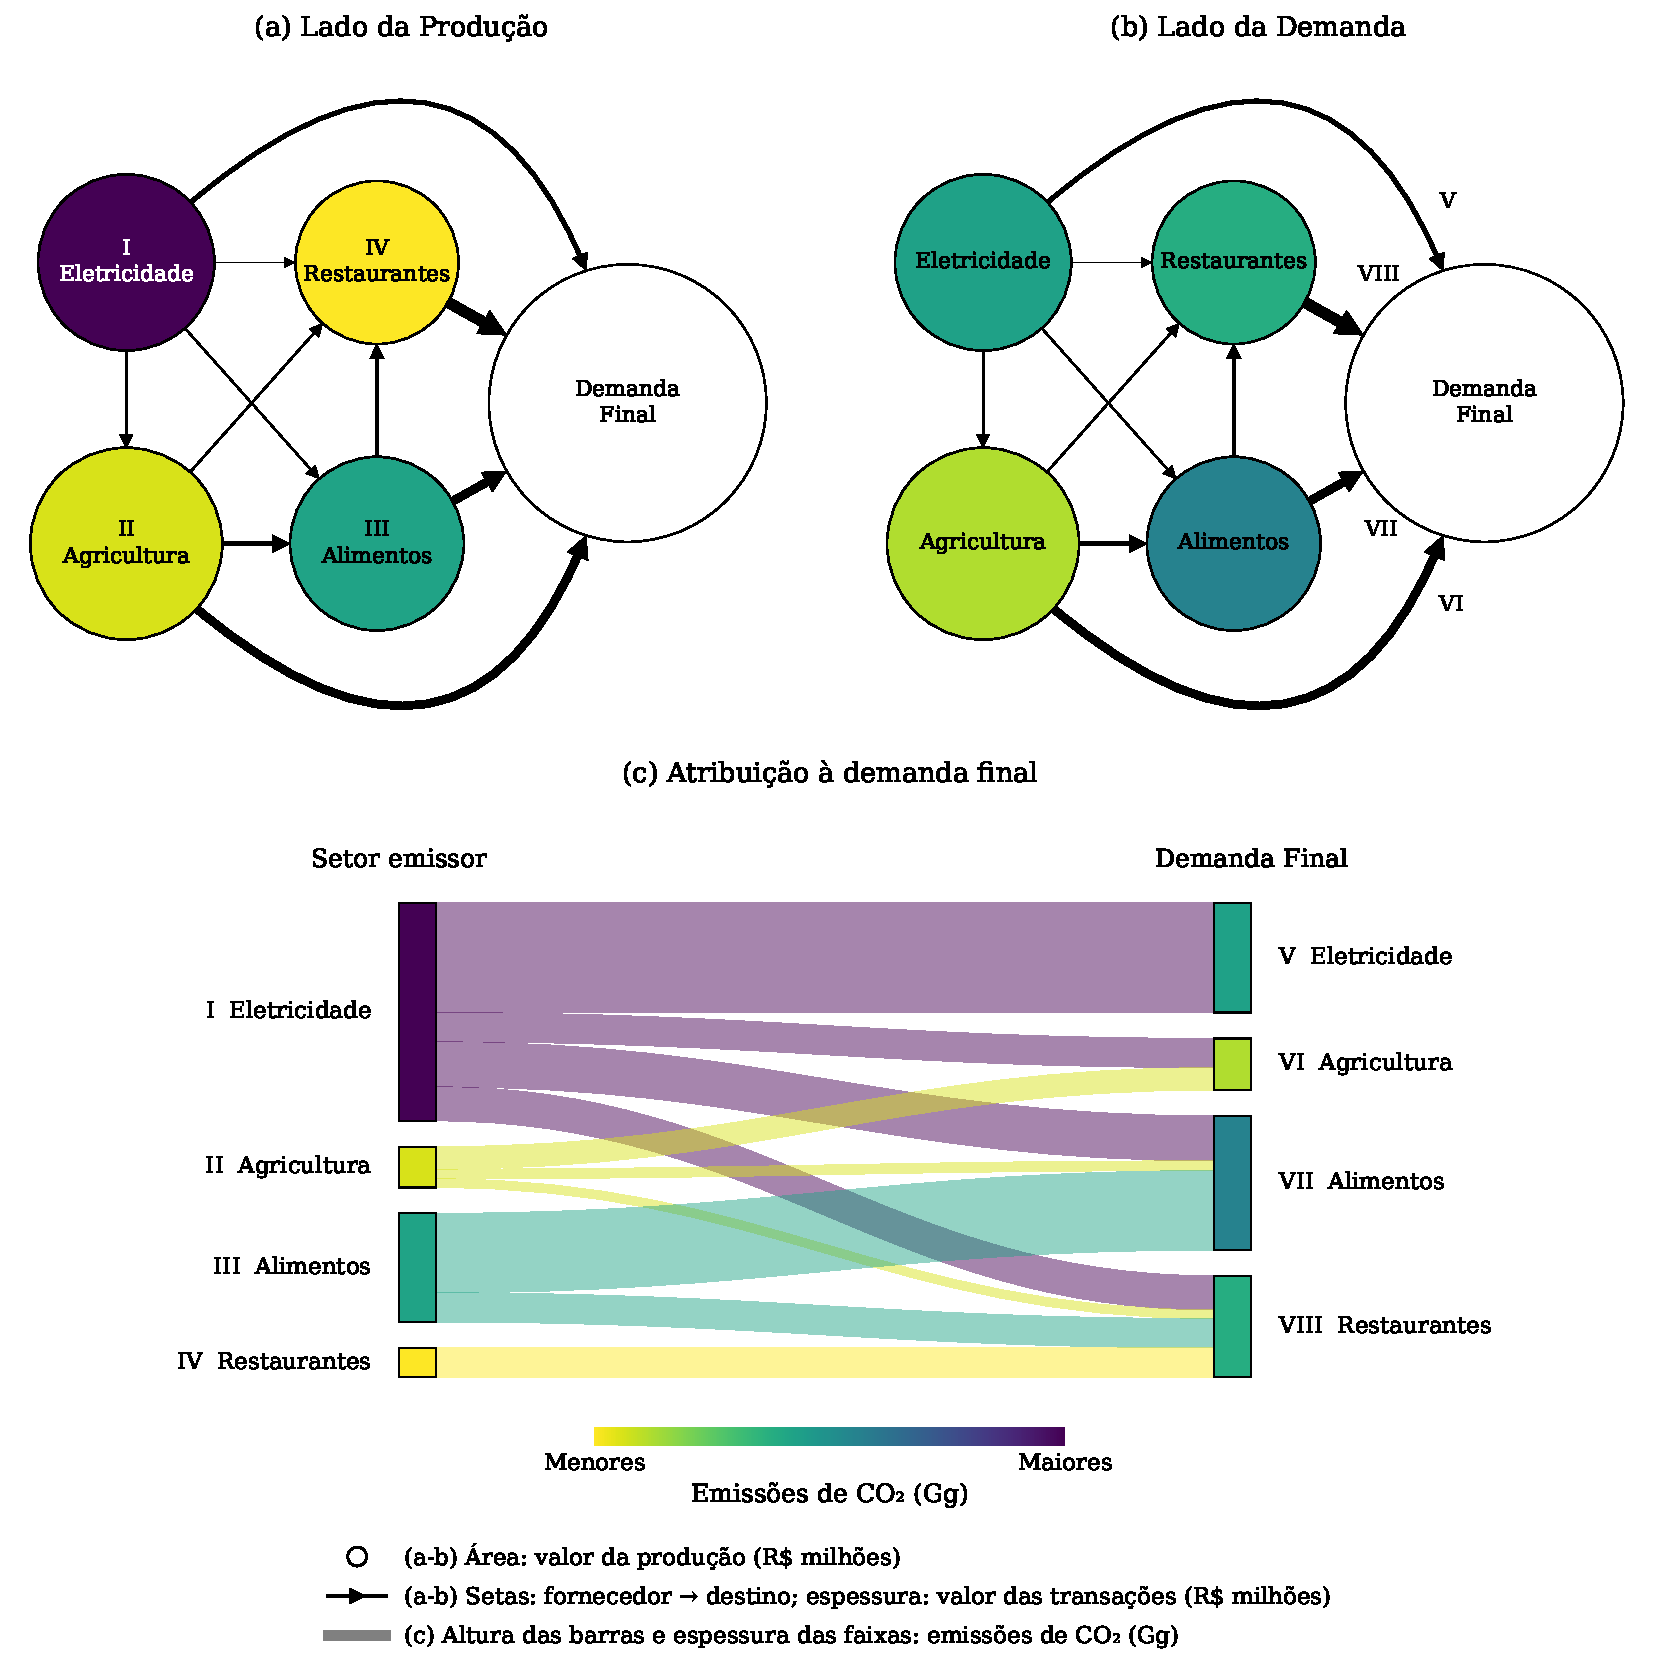
\includegraphics[width=\textwidth,height=0.7\textheight,keepaspectratio]{figuras/atribuicao_cadeia_alimentos.pdf}
\caption{Exemplo detalhado das atribuições em uma economia didática de quatro atividades.}
\label{fig:exemplo-detalhado}
\begin{minipage}{\textwidth}\footnotesize
Fonte: elaboração própria, figura preservada da versão anterior. Em (a--b), áreas e setas indicam valores monetários e as cores distinguem produção e demanda. Em (c), as faixas indicam atribuições de emissões entre origens e produtos finais. Exemplo didático, sem estimativas nacionais.
\end{minipage}
\end{figure}
\subsection{Construção da rede dirigida e ponderada}
\label{sec:construcao-rede}

A rede tem 67 nós, um por atividade da MIP, identificados pelos códigos do IBGE. Cada nó representa uma origem emissora nas ligações de saída e o setor de um produto final nas ligações de entrada, seguindo a representação de atribuição de \textcite{huang2019}. Os dois papéis pertencem ao mesmo nó, enquanto o Sankey da Figura~\ref{fig:exemplo-detalhado} os apresenta em conjuntos separados.

Para estudar relações entre atividades distintas, define-se
\begin{equation}
W_{ij}=\begin{cases}
F_{ij}, & i\ne j,\\
0, & i=j.
\end{cases}
\label{eq:rede-sem-diagonal}
\end{equation}
Há uma aresta $i\rightarrow j$ para cada $W_{ij}>0$, com peso igual a esse valor, em Gg de CO\textsubscript{2}. A direção indica a origem emissora e o destino da atribuição, e as duas direções de um par serão tratadas separadamente. Como os pesos já incorporam requisitos diretos e indiretos, concatenar essas arestas não representa uma sequência de etapas produtivas.

A diagonal $F_{ii}$ reúne emissões de $i$ atribuídas à demanda final de seus próprios produtos, incluindo os requisitos indiretos correspondentes. Ela permanece nas contas $c$ e $u$, mas é retirada de $W$ para separar as relações entre atividades da atribuição à própria atividade. Assim, $W$ não terá laços, e seu peso total corresponderá apenas à parcela intersetorial das emissões.

São mantidos todos os nós e todas as arestas positivas, sem corte por magnitude nesta etapa. A construção exige alinhamento dos códigos e pesos finitos e não negativos; eventuais valores negativos são examinados antes da representação, sem conversão automática para zero ou valor absoluto. A seleção de arestas será tratada na seção~\ref{sec:backbone}.

\subsection{Volume e concentração das relações}
\label{sec:volume-concentracao}

Para relacionar a estrutura da rede às duas contas ambientais, são examinados o volume das relações externas e sua distribuição entre contrapartes. As medidas são calculadas em $W$, antes da filtragem, com referência às forças de \textcite{huang2019} e à disparidade dos pesos de \textcite{serrano2009}.

\paragraph{Volume.}
As forças de saída e entrada são as somas dos pesos em cada direção:
\begin{equation}
\begin{aligned}
s_i^{\mathrm{out}}&=\sum_{j\ne i}W_{ij}=c_i-F_{ii},\\
s_i^{\mathrm{in}}&=\sum_{j\ne i}W_{ji}=u_i-F_{ii}.
\end{aligned}
\label{eq:forcas-externas}
\end{equation}
A saída mede as emissões próprias de $i$ atribuídas aos produtos finais de outras atividades; a entrada mede as emissões de outras atividades atribuídas aos produtos finais de $i$. Ambas têm unidade de Gg de CO\textsubscript{2}. Sua diferença é $u_i-c_i$, mas a leitura separada permite identificar grandes volumes que se compensam no saldo. São apresentados também $c_i$, $u_i$ e $F_{ii}$, para situar a parcela intersetorial em cada conta completa.

\paragraph{Concentração.}
Para perfis com força positiva, define-se a participação de cada contraparte:
\begin{equation}
p_{ij}^{\mathrm{out}}=\frac{W_{ij}}{s_i^{\mathrm{out}}},\qquad
p_{ji}^{\mathrm{in}}=\frac{W_{ji}}{s_i^{\mathrm{in}}},\quad j\ne i.
\label{eq:participacoes-externas}
\end{equation}
O perfil de saída distribui as emissões externas da origem entre destinos; o de entrada descreve as origens que compõem a atribuição externa ao destino. Cada perfil soma um. A disparidade e seu inverso são calculados por
\begin{equation}
\begin{aligned}
Y_i^{\mathrm{out}}&=\sum_{j\ne i}(p_{ij}^{\mathrm{out}})^2,&
Y_i^{\mathrm{in}}&=\sum_{j\ne i}(p_{ji}^{\mathrm{in}})^2,\\
D_{2,i}^{\mathrm{out}}&=1/Y_i^{\mathrm{out}},&
D_{2,i}^{\mathrm{in}}&=1/Y_i^{\mathrm{in}}.
\end{aligned}
\label{eq:disparidade}
\end{equation}
$Y$ aumenta com a concentração; $D_2$ expressa a mesma informação como número efetivo de contrapartes. Para $k$ pesos iguais, $D_2=k$; quando uma relação domina, aproxima-se de um. Essas medidas são adimensionais e ficam indefinidas quando a força é zero, sem excluir o nó da análise.

A combinação de força e número efetivo permite distinguir volumes elevados concentrados em poucas contrapartes de volumes distribuídos entre muitas. As atividades que compõem cada perfil são identificadas pelos pesos e participações, pois o número efetivo não informa sua identidade. O grau conta as arestas positivas de entrada ou saída; a densidade é o número de arestas dividido por $67\times66$. Grau e densidade descrevem a presença de relações, enquanto a disparidade considera a distribuição de seus pesos.

\subsection{Extração e avaliação do backbone}
\label{sec:backbone}

O filtro de disparidade de \textcite{serrano2009}, aplicado por \textcite{huang2019}, é utilizado para selecionar ligações destacadas na composição local dos pesos. A seleção depende da participação da aresta na força de cada extremidade, permitindo considerar atividades de diferentes escalas. Seu resultado será o backbone, sem alterar as contas ambientais completas.

\paragraph{Critério de seleção.}
O modelo nulo divide o intervalo unitário em $k$ parcelas por $k-1$ pontos escolhidos uniformemente, representando uma distribuição aleatória da força entre as ligações. Para $k>1$, a probabilidade de uma parcela atingir ou superar $p$ é $(1-p)^{k-1}$. Para a aresta $i\rightarrow j$, as caudas nas perspectivas de saída e entrada são
\begin{equation}
\begin{aligned}
a_{ij}^{\mathrm{out}}&=\left(1-\frac{W_{ij}}{s_i^{\mathrm{out}}}\right)^{k_i^{\mathrm{out}}-1},\\
a_{ij}^{\mathrm{in}}&=\left(1-\frac{W_{ij}}{s_j^{\mathrm{in}}}\right)^{k_j^{\mathrm{in}}-1}.
\end{aligned}
\label{eq:caudas-filtro}
\end{equation}
Os graus $k$ e as forças são os de $W$. A aresta é selecionada se $a_{ij}^{\mathrm{out}}<\alpha$ \textbf{ou} $a_{ij}^{\mathrm{in}}<\alpha$, registrando-se qual extremidade determina a seleção. A saída destaca um destino nas atribuições da origem; a entrada destaca uma origem na composição do destino.

As caudas só são calculadas para graus pertinentes maiores que um. Se apenas uma extremidade tiver grau um, vale o teste da outra; se ambas tiverem grau um, a aresta é preservada por convenção de manutenção da relação exclusiva, inclusive em díades isoladas. Essa extensão dos casos degenerados do suplemento de Serrano et al. é registrada separadamente da seleção estatística. Todos os nós são mantidos.

Adota-se $\alpha=0{,}05$, com $0{,}01$ e $0{,}10$ para sensibilidade. Para cada valor, o filtro é aplicado uma vez a $W$, sem atualização iterativa dos perfis. A matriz resultante $B_\alpha$ mantém os pesos originais nas arestas selecionadas e zero nas demais, sem renormalização ou corte absoluto adicional.

\paragraph{Avaliação da seleção.}
São comparadas a fração de arestas retidas e a cobertura dos pesos, globalmente e por atividade:
\begin{equation}
\begin{aligned}
r_\alpha&=\frac{\sum_{ij}(B_\alpha)_{ij}}{\sum_{ij}W_{ij}},\\
r_{\alpha,i}^{\mathrm{out}}&=\frac{\sum_j(B_\alpha)_{ij}}{s_i^{\mathrm{out}}},\qquad
r_{\alpha,i}^{\mathrm{in}}=\frac{\sum_j(B_\alpha)_{ji}}{s_i^{\mathrm{in}}}.
\end{aligned}
\label{eq:cobertura-backbone}
\end{equation}
As razões serão definidas apenas para denominadores positivos. A cobertura se refere à parcela intersetorial de $W$; sua leitura por atividade permite identificar perdas ocultas pela retenção agregada. São descritos também graus, forças retidas, isolados e componentes fracamente conectados, obtidos ao desconsiderar a direção das arestas para verificar conectividade.

A sensibilidade é examinada pelas mudanças nas arestas, coberturas e posições setoriais entre os três valores de $\alpha$. Com convenções fixas, os conjuntos são aninhados por construção; essa propriedade não constitui evidência independente de robustez. O modelo nulo é uma referência de distribuição dos pesos: suas caudas não medem a incerteza ambiental, e a seleção não estabelece prioridade de mitigação.

A resposta à pergunta combina as contas e seus saldos em $F$, os volumes e a concentração em $W$ e as contrapartes destacadas em $B_\alpha$. As relações são interpretadas junto de seus pesos e coberturas: uma ligação pode ser importante localmente e pequena no total, enquanto uma ligação não selecionada continua integrando a contabilidade. Assim, o backbone complementa a análise dos perfis completos, sem substituí-los.

